%%%%%%%%%%%%%%%%%%%%%%%%%%%%%%%%%%%%%%%%%
% Engineering Calculation Paper
% LaTeX Template
% Version 1.0 (20/1/13)
%
% This template has been downloaded from:
% http://www.LaTeXTemplates.com
%
% Original author:
% Dmitry Volynkin (dim_voly@yahoo.com.au)
%
% License:
% CC BY-NC-SA 3.0 (http://creativecommons.org/licenses/by-nc-sa/3.0/)
%
%%%%%%%%%%%%%%%%%%%%%%%%%%%%%%%%%%%%%%%%%

%----------------------------------------------------------------------------------------
%	PACKAGES AND OTHER DOCUMENT CONFIGURATIONS
%----------------------------------------------------------------------------------------

\documentclass[12pt,a4paper]{article} % Use A4 paper with a 12pt font size - different paper sizes will require manual recalculation of page margins and border positions
\usepackage[utf8]{inputenc}
\usepackage{marginnote} % Required for margin notes
\usepackage{wallpaper} % Required to set each page to have a background
\usepackage{lastpage} % Required to print the total number of pages
\usepackage[left=1.3cm,right=1.3cm,top=1.8cm,bottom=2.2cm,marginparwidth=3.4cm]{geometry} % Adjust page margins
\usepackage[fleqn]{amsmath} % Required for equation customization
\usepackage{amssymb} % Required to include mathematical symbols
\usepackage{xcolor} % Required to specify colors by name
\usepackage{xfrac}
\usepackage{fancyhdr} % Required to customize headers
\usepackage{booktabs}
\usepackage{xargs}
\setlength{\headheight}{12mm} % Increase the size of the header to accommodate meta-information
\pagestyle{fancy}\fancyhf{} % Use the custom header specified below
\renewcommand{\headrulewidth}{0pt} % Remove the default horizontal rule under the header

\setlength{\parindent}{0cm} % Remove paragraph indentation
\newcommand{\tab}{\hspace*{2em}} % Defines a new command for some horizontal space

\newcommand\BackgroundStructure{ % Command to specify the background of each page
	\setlength{\unitlength}{1mm} % Set the unit length to millimeters

	\setlength\fboxsep{0mm} % Adjusts the distance between the frameboxes and the borderlines
	\setlength\fboxrule{0.25mm} % Increase the thickness of the border line
	%%\put(10, 15){\fcolorbox{black}{white!10}{\framebox(150,260){}}} % Main content box
	%%\put(150, 15){\fcolorbox{black}{gray!10}{\framebox(45,260){}}} % Margin box
%%	\put(10, 278){\fcolorbox{black}{white!10}{\framebox(192, 12){}}} % Header box
%% \put(137, 263){\includegraphics[height=23mm,keepaspectratio]{logo}} % Logo box - maximum height/width: 
}
\newcommand\const{\mathrm{const}}
\newcommand\solve[2]{\text{solve}\left\(#1\;\text{pour}\;#2\right\)}
%% \newcommand\vec\overrightarrow

%----------------------------------------------------------------------------------------
%	HEADER INFORMATION
%----------------------------------------------------------------------------------------

\fancyhead[L]{
	{\LARGE Formulaire de physique}
}
\fancyfoot[R]{
	{\small \thepage/\pageref{LastPage}}
}


%----------------------------------------------------------------------------------------

\begin{document}

\newcommand\formula[2]{#1 & = & #2}
\newcommand\nextcol{}
\newenvironmentx{twocols}[2][1=0.5, 2=0.4]{
	\def\colonewidth{#1}
	\def\coltwowidth{#2}
	\renewcommand\nextcol{
		\vspace{0.4em}
		\end{minipage}
		\vrule\quad
		\begin{minipage}[t]{\coltwowidth\textwidth}
		\vspace{0.4em}
	}
	\begin{minipage}[t]{\colonewidth\textwidth}
	\vspace{0.4em}
}{
	\vspace{0.4em}
	\end{minipage}

}

\AddToShipoutPicture{\BackgroundStructure} % Set the background of each page to that specified above in the header information section

%----------------------------------------------------------------------------------------
%	DOCUMENT CONTENT
%----------------------------------------------------------------------------------------

\section{Mouvements}

\subsection*{General}

\textbf{Unités} \\
\begin{math}
	\begin{array}{rl}
		a & \sfrac{m}{s^2} \\
		v & \sfrac{m}{s} \\
		x & m \\
	\end{array}
\end{math}


\subsection*{Mouvement Rectiligne (MRU \& MRUA)}
\begin{twocols}[0.7][0.2]
	MRU
	\begin{equation*}
	\left\{
		\begin{array}{r c l}
			\formula{v}{\const} \\
			\formula{x}{x_0 + v t} \\
		\end{array}
	\right.
	\end{equation*}
	\par\vspace{1em}
	MRUA \\
	\begin{equation*}
	\left\{
		\begin{array}{rcl}
			\formula{a}{\const} \\
			\formula{v(t)}{a t} \\
			\formula{x(t)}{x_0 + v_0 * t + \frac{a t^2}{2}} \\
		\end{array}
	\right.
	\end{equation*}

\nextcol
	
	\begin{tabular}{r l}
		x & \text{Position} \\
		v & \text{Vitesse} \\
		a & \text{Accélération} \\
	\end{tabular}
	


\end{twocols}

\subsection*{Mouvement Circulaire (MCU \& MCUA)}
\begin{twocols}[0.7][0.2]
	MCU
	\begin{equation*}
	\left\{
		\begin{array}{rcl}
			\formula{\omega}{\const} \\
			\formula{\theta}{\omega t + \theta_0} \\
		\end{array}
	\right.
	\end{equation*}
	\par\vspace{1em}
	MCUA
	\begin{equation*}
	\left\{
		\begin{array}{rcl}
			\formula{\alpha}{\const} \\
			\formula{\omega}{\omega_0 + \alpha t} \\
			\formula{\theta}{\theta_0 + \omega t + \frac{\alpha t^2}{2}} \\
		\end{array}
	\right.
	\end{equation*}

\nextcol


	\begin{tabular}{rl}
		$\theta$ & Angle \\
		$\omega$ & Vitesse \\
		$\alpha$ & Accélération \\
	\end{tabular}

\end{twocols}

\newpage

\section{Balistique}
\begin{figure*}
	\centering
	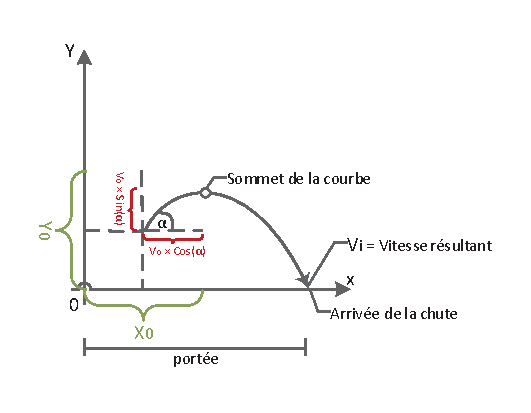
\includegraphics[width=0.5\textwidth]{images/Balistique}	
\end{figure*}

\begin{twocols}
	Acceleration
	\begin{equation*}
	\left\{
		\begin{array}{rcl}
			\formula{a_x}{0} \\
			\formula{a_y}{-g\;\text{OU}\;\const} \\
		\end{array}
	\right.
	\end{equation*}
	\par\vspace{1em}
	Vitesse
	\begin{equation*}
	\left\{
		\begin{array}{rcl}
			\formula{v_x(t)}{v_0\,\cos{\alpha}} \\
			\formula{v_y(t)}{v_0\,\sin{\alpha}-a_y\,t^2} \\
		\end{array}
	\right.
	\end{equation*}
	Position
	\begin{equation*}
	\left\{
		\begin{array}{rcl}
			\formula{x_x(t)}{x_0+v_0\,\cos{\alpha}\,t} \\
			\formula{x_y(t)}{y_0+v_0\,\cos{\alpha}\,t-\frac{a\,t^2}{2}} \\
		\end{array}
	\right.
	\end{equation*}

\nextcol
	
	Port\'ee
	\begin{equation*}
		\left\{
		\begin{array}{ll}
			p=\frac{v_0^2\,\sin{2\alpha}}{a} & \text{Si}\:y_0 = 0 \\
			p=\text{solve}\left(\left\{
					\begin{array}{rcl}
						y(t) & = & 0 \\
						x(t) & = & n \\
					\end{array}
			\right|
				\text{en} \: n
			\right)
			 & \text{Si}\:y_0 \neq 0
		\end{array}
		\right.
	\end{equation*}

	Alt. Maximale
	\begin{equation*}
		y_\text{max} = \frac{(v_0\,\sin{\alpha})^2}{2a} + y_0
	\end{equation*}

\end{twocols}

\newpage
\section{Statique}
\begin{twocols}
	\subsection*{Somme des forces}

	\begin{equation*}
		\sum \vec{F} = 0
	\end{equation*}

\nextcol
	
	En statique la somme des forces s'\'equilibre toujours

\end{twocols}
\begin{twocols}
	\subsection*{Moment de Force}

	\begin{equation*}
		M_o = F \times d
	\end{equation*}

\nextcol

	Projection de la force $F$ situ\'e \`a $d$ sur $O$ en $M_o$

\end{twocols}

\section{Transfert de chaleur}

\begin{twocols}
	
\begin{equation*}
	\begin{array}{r c l}
		\formula{\sum{Q}}{0} \\
		\formula{Q}{m\,c\,\Delta\theta} \\
		\formula{Q}{m\,C} \\
		\formula{\Delta\theta}{T_2 - T_2} \\
	\end{array}
\end{equation*}

\nextcol

	\begin{tabular}{rl}
		$Q$ & Energie [J] \\
		$\Delta\theta$ & Diff. de temperature [C]\\
		$m$ & Masse [kg] \\
		$c$ & Chaleur specifique \\
		$C$ & Coefficient de transformation
	\end{tabular}


\end{twocols}

%----------------------------------------------------------------------------------------

\end{document}